\section*{Код программы}
В файле hello\_world\_small.c находится доработанный код эхо-программы приёма-передачи по интерфейсу RS232.

Также был создан образ OC HAL с драйверами устройств, используемых в аппаратном проекте.

На листинге 1 приведён код программы по заданию.

\FloatBarrier
\begin{lstinputlisting}[language=C++, caption=Код для выполнения задания, 
	linerange={1, 16}, basicstyle=\footnotesize\ttfamily, frame=single, breaklines=true]{src/main.cpp}
\end{lstinputlisting}
\FloatBarrier

В результате получилось окно, представленное на рисунке 6.

\FloatBarrier
\begin{figure}[h]
	\begin{center}
		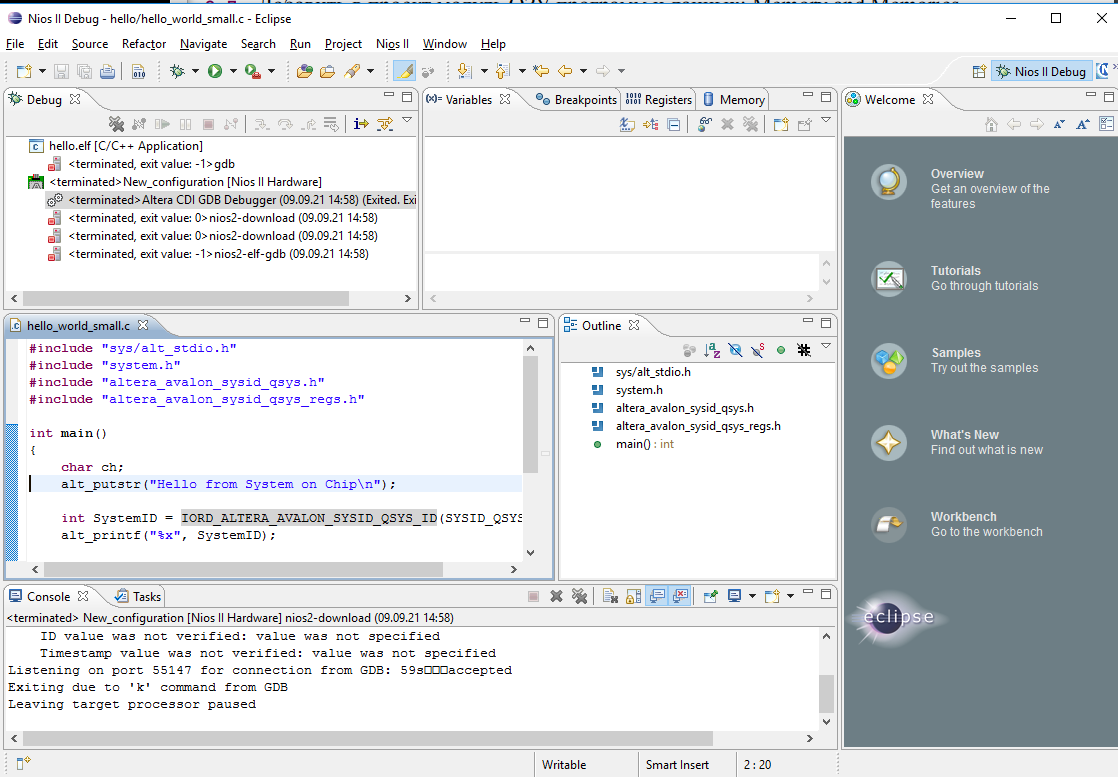
\includegraphics[width=\linewidth]{inc/codeResult.png}
	\end{center}
	\caption{Итоговый результат проекта Nios II}
\end{figure}
\FloatBarrier